\documentclass[aspectratio=169]{beamer}
\usepackage[utf8]{inputenc}
\usepackage[T1]{fontenc}
\usepackage{lmodern}
\usepackage{listings}
\usepackage{xcolor}
\usepackage{graphicx}
\usepackage{booktabs}
\usepackage{verbatim}

% Theme and color scheme
\usetheme{Madrid}
\usecolortheme{default}

% Code highlighting
\lstset{
    language=C++,
    basicstyle=\ttfamily\small,
    keywordstyle=\color{blue}\bfseries,
    commentstyle=\color{green!60!black},
    stringstyle=\color{red},
    numberstyle=\tiny\color{gray},
    numbers=left,
    breaklines=true,
    showstringspaces=false,
    frame=single,
    backgroundcolor=\color{gray!10}
}

% Title page information
\title{Introduction to Intrusive \& Visual Profiling}
\subtitle{Focusing on Constrained Environments}
\author{Lukáš Růžička}
\institute{Prague C++ Meetup}
\date{2025 07 29}



\begin{document}



% Title slide
\frame{\titlepage}

\begin{frame}{Table of Contents}
\tableofcontents[hideallsubsections]
\end{frame}

% Current section
\AtBeginSection[ ]
{
\begin{frame}{Outline}
    \tableofcontents[currentsection]
\end{frame}
}



\section{Personal introduction}

\begin{frame}
    Ahoj, ja jsem Lukas.

    Prosim, otazky klidne pokladejte hned, ci si je nechte na konec (idealne si zapamatujte kontext pomoci cisla stranky, dole v rohu).

    Libi se mi "koncept" techto meetupu, a rikal jsem si, ze bych rad prispel, ne jen "konzumoval" prednasky ostatnich. Ale cim (viz nize), a jak (viz domluva na discord serveru, proklik z https://www.meetup.com/prague-cpp/)?

    Jeden ze svych prvnich ukolu (je to cca 7 let zpatky, detaily si nepamatuju) ve sve programatorske kariere jsem pomoci nej vyresil za pomoci knihovny `nvtx' a nejakeho addonu do `Visual studio', ktery ta data "prijimal" a zobrazoval.

    Slo o to, ze jedno vlakno pushovalo do fronty, a druhe z ni popovalo. Kdyz byla fronta prazdna, tak tam byl "timed wait", asi pomoci `std::condition\_variable' ci obdobneho. Ten byl volan nejak neoptimalne (ci rovnou uplne spatne), a nikdy nedoslo k jeho ukonceni jinak nez timeoutem, coz jsem tenkrat krasne vypozoroval z vysledku daneho profilovani.

    Profilovani mi prijde zajimave a zabavne.

\end{frame}



\section{Content of the talk}

\begin{frame}
    Jak to pojmout? Mel jsem predstavu, ktera se setkala s pozitivnim ohlasem (TODO zminit to konkretni vlakno s tim "poll"em):

    \begin{itemize}
        \item nejdrive popsat svou zkusenost s "externimi" knihovnami/frameworky/nastroji:
        \begin{itemize}
            \item `nvtx' TODO link zde nebo pozdeji?!
            \item `Tracy' TODO ditto
            \item `perf' + `flamegraphs' ...
        \end{itemize}
        \item zminit nejake dalsi (o kterych jsem "slysel", ale nikdy je nepouzival):
        \begin{itemize}
            \item `Intel VTune Profiler' ...
            \item `Clang XRay' https://llvm.org/docs/XRay.html ...
        \end{itemize}
        \item pak zminit v cem mi nevyhovovaly a co jsem potreboval jinak.
        \item Z toho vyplynulo, ze jsem zacal psat "vlastni" knihovnu pro tento ucel (`cxxet', viz https://github.com/Ruzovej/cxxet).
    \end{itemize}

\end{frame}



\section{Vysvetleni pojmu}

\begin{frame}{Application profiling}
    To profile an application means to somehow measure its performance, resource usage, etc. in order to identify bottlenecks, potential optimization opportunities, and so on.

    Some related quotes:
    \begin{itemize}
        \item "Premature optimization is root of all evil."
        \item "You don't improve what you don't measure."
    \end{itemize}

\end{frame}

\begin{frame}{Non-intrusive profiling}
    Measuring which doesn't require any source code (of target application) modification. This is usually done by attaching some tool to the running application, which then collects data about its performance, resource usage, and so on.

    Examples:

    \begin{itemize}
        \item `time ...' - the simplest and crudest option (for unix OSes)
        \item `perf' (in tandem with `Flame Graph' tools for the "visual" part)
        \item Microsoft Visual Studio Profiler (e.g. https://learn.microsoft.com/en-us/visualstudio/profiling)
    \end{itemize}

\end{frame}

\begin{frame}{Intrusive profiling}
    Je specificke modifikaci zdrojoveho kodu programu - zpravidla postupne pridavani markeru/logovani/apd. na zaklade vysledku z predchozi iterace.

    Je velmi podobne takzvanemu "printf debugging", ktere zaroven muze byt pouzito jako nejjednodussi profilovani tohoto druhu - vypis zmerenych casu na standartni vystup, do logu, a podobne.

\end{frame}

\begin{frame}{Visual profiling}
    Zobrazeni vysledku pomoci nejakeho UI, napriklad `chrome://tracing' (TODO obrazek) ci perfetto.ui (TODO link a obrazek).

    Opakem muze byt "zakladni" (napr. textove) zobrazeni vysledku jako napriklad `perf report' (TODO obrazek ci ukazka?!), nebo pouhe logovani casu stravenych v nejake casti kodu.

\end{frame}

\begin{frame}{Constrained environments}
    Omlouvam se za trochu zavadejici nazev - konkretne za to slovo "constrained" - obecne je v oboru softwaroveho vyvoje chapano ve spojitosti s embedded, ale to nebyl muj pripad - moje prostredi byl sice "velky" server, ale omezeni byla jina - absence `root' pristupu (pro perf) a vnitrni architektura aplikace.

\end{frame}



\section{Zavedene nastroje, knihovny a frameworky}


\subsection{Nvtx}

\begin{frame}[fragile]{Nvtx usage example}{example code `examples/nvtx/main.cxx'}
    
    \begin{lstlisting}[language=C++]
#include <thread>
#include <nvtx3/nvtx3.hpp>

void some_function() {
  NVTX3_FUNC_RANGE(); // equivalent to e.g. `nvtx3::scoped_range fn{__FUNCTION__};'
  for (int i = 0; i < 6; ++i) {
    nvtx3::scoped_range loop{"loop iteration range"};
    // Make each iteration last for one ms:
    std::this_thread::sleep_for(std::chrono::milliseconds{1});
  }
}

int main(int, char **) {
  some_function();
}
    \end{lstlisting}

\end{frame}

\begin{frame}{Nvtx usage example}
    Windows host, linux target:

    \begin{enumerate}
        \item download and install it on windows host: https://developer.nvidia.com/nsight-systems/get-started\#Winx86
        \item download it for linux target (e.g. Ubuntu): https://developer.nvidia.com/nsight-systems/get-started\#Linuxx86
        \item install it: `sudo dpkg --install NsightSystems-linux-cli-public-2025.3.1.90-3582212.deb'
        \item compile the example: `\$ cd examples/nvtx \&\& ./build.bash'
        \item run it: `\$ time nsys profile build/nvtx\_example'
        \item add/remove markers in source code as needed
        \item go to step no. 4, etc.
    \end{enumerate}

\end{frame}

\begin{frame}{Nvtx usage example}{example output}
    \begin{figure}[h]
        \centering
        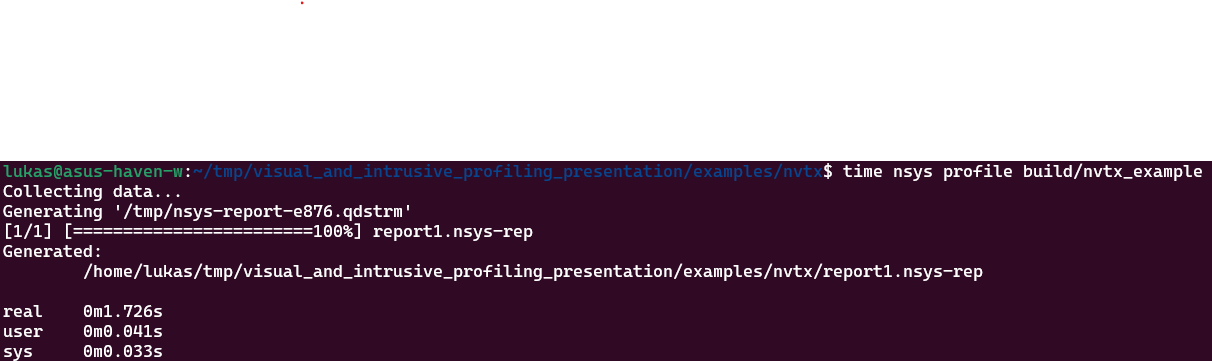
\includegraphics[width=\textwidth,height=0.7\textheight,keepaspectratio]{pics/nvtx/nsys_example.png}
        \caption{Application profiling via nsys and nvtx}
    \end{figure}

\end{frame}

\begin{frame}{Nvtx usage example}{displayed data}

    \begin{figure}[h]
        \centering
        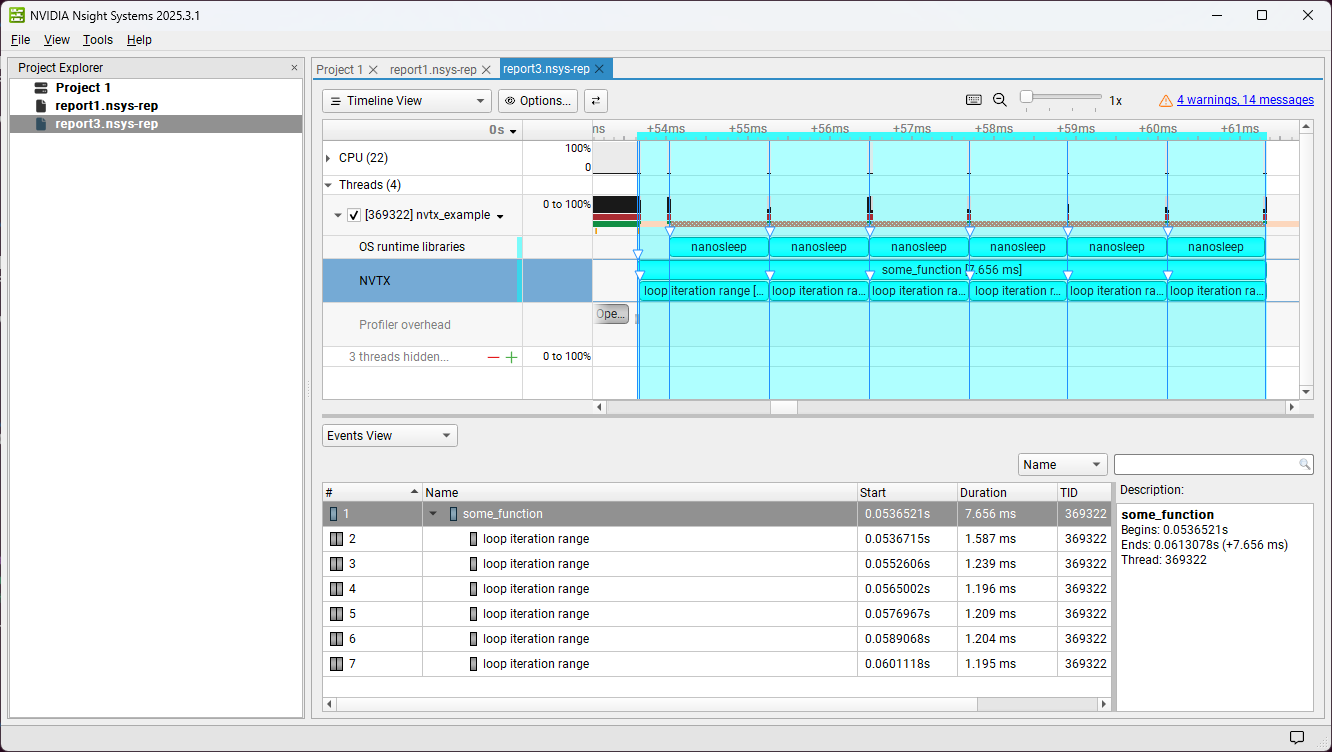
\includegraphics[width=\textwidth,height=0.7\textheight,keepaspectratio]{pics/nvtx/gui.png}
        \caption{Nsight Systems profiling gui}
    \end{figure}

\end{frame}

\begin{frame}{NVIDIA Nsight Systems + nvtx}
    Odkazy (TODO mozna je dat na konec tohoto slide):

    \begin{itemize}
         \item https://developer.nvidia.com/nsight-systems
         \item https://docs.nvidia.com/nsight-systems/UserGuide/index.html\#nvtx-trace
         \item https://github.com/NVIDIA/NVTX
    \end{itemize}

    Vyhody:

    \begin{itemize}
        \item velmi rozsahly framework, umi to daleko vic veci nez co tu popisuji
        \item moznost sledovat chovani v realnem case (pri spusteni prez gui)
    \end{itemize}

    Nevyhody:

    \begin{itemize}
        \item profiler (`nsys' v prikladu vyse) je samostatna aplikace, ktera pokud neni vyhovujici/dostupna, je nutnost "dodat" svoji implementaci (viz. https://github.com/NVIDIA/NVTX/tree/release-v3/tools/sample-injection)
    \end{itemize}

\end{frame}


\subsection{Tracy}

\begin{frame}[fragile]{Tracy usage example}{example code `examples/tracy/main.cxx'}
    
    \begin{lstlisting}[language=C++]
#include <thread>
#include <tracy/Tracy.hpp>

void some_function() {
  ZoneScoped; // equivalent to the `NVTX3_FUNC_RANGE();`
  for (int i = 0; i < 6; ++i) {
    ZoneScopedN("loop iteration range"); // equivalent to the
                                         // `nvtx3::scoped_range loop{...};`
    std::this_thread::sleep_for(std::chrono::milliseconds{1});
  }
}

int main(int, char **) { some_function(); }
    \end{lstlisting}

\end{frame}

\begin{frame}{Tracy usage example}
    All on linux (wsl2 Ubuntu):

    \begin{enumerate}
        \item build its gui (see section 2.3 in its documentation):
        \begin{itemize}
            \item `\$ cmake -B profiler/build -S profiler -DCMAKE\_BUILD\_TYPE=Release -DLEGACY=ON'
            \item `\$ cmake --build profiler/build --config Release --parallel'
        \end{itemize}
        \item compile the example: `\$ cd examples/tracy \&\& ./build.bash'
        \item run it: `\$ TRACY\_NO\_EXIT=1 build/tracy\_example'
        \item drain the collected data via gui `\$ profiler/build/tracy-profiler' and explore it
        \item adjust markers in the source code as needed
        \item repeat if needed: go to step no. 3
    \end{enumerate}

\end{frame}

\begin{frame}{Tracy usage example}{fresh gui}
    \begin{figure}[h]
        \centering
        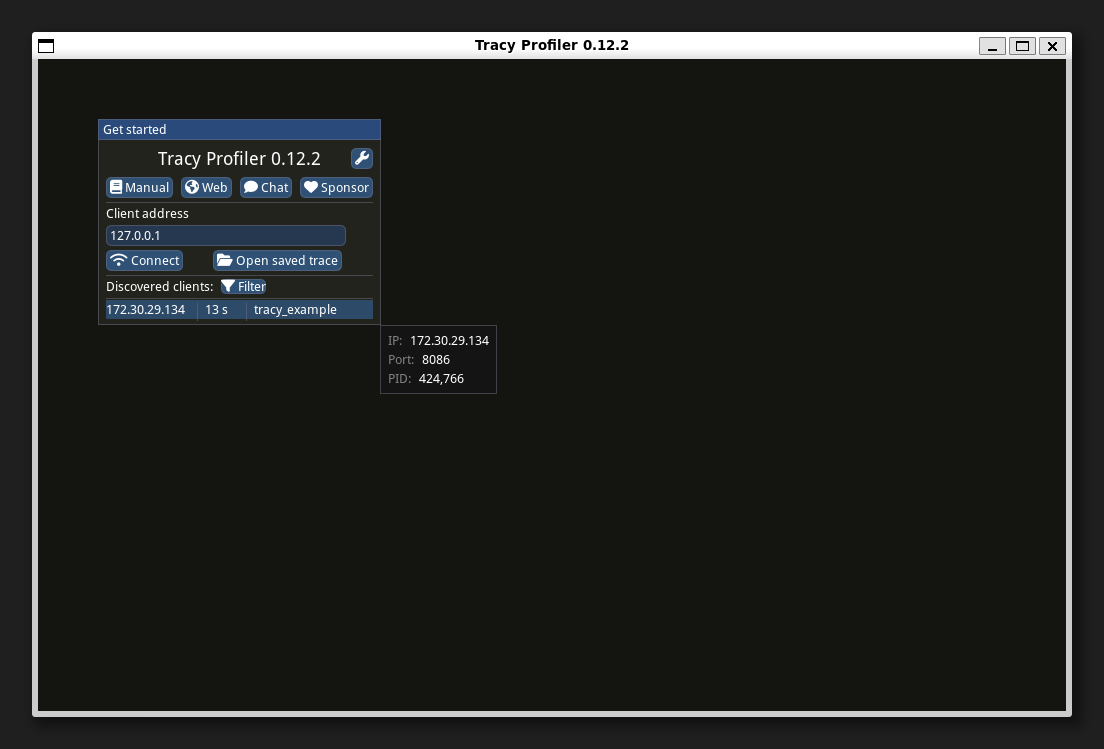
\includegraphics[width=\textwidth,height=0.7\textheight,keepaspectratio]{pics/tracy/gui1.png}
        \caption{Choosing process}
    \end{figure}

\end{frame}

\begin{frame}{Tracy usage example}{displayed data}

    \begin{figure}[h]
        \centering
        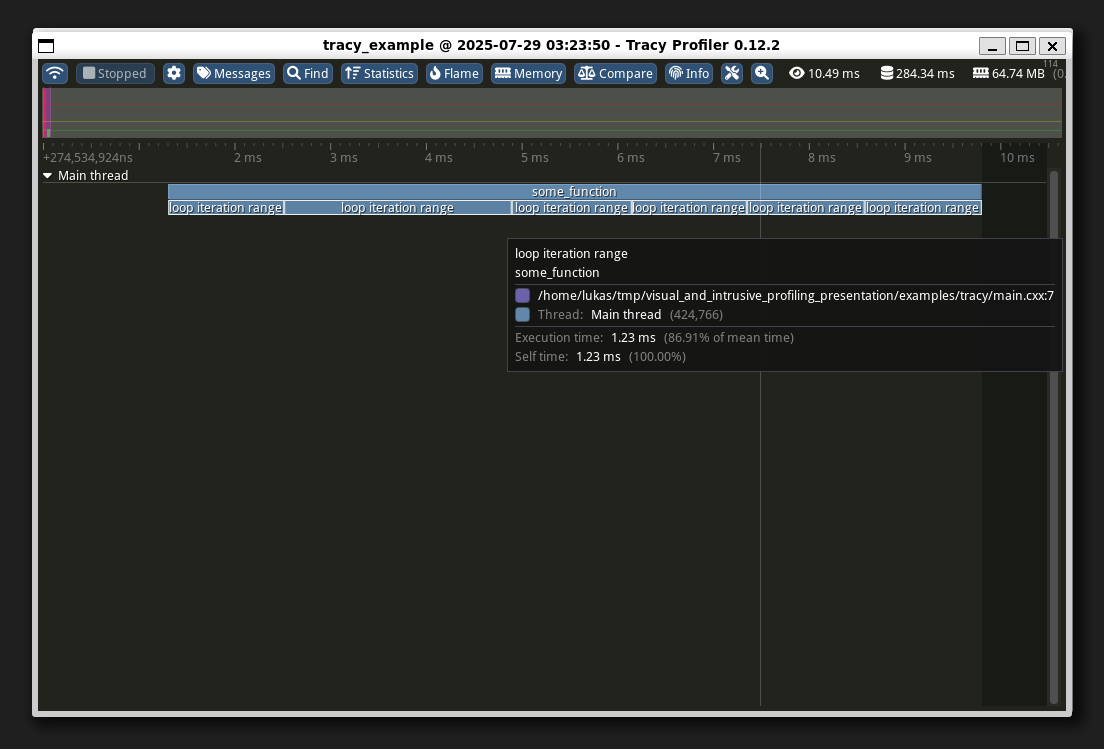
\includegraphics[width=\textwidth,height=0.7\textheight,keepaspectratio]{pics/tracy/gui2.png}
        \caption{Tracy gui}
    \end{figure}

\end{frame}

\begin{frame}{Tracy}
    Odkazy (TODO mozna je dat na konec tohoto slide):

    \begin{itemize}
        \item https://github.com/wolfpld/tracy
        \item https://github.com/wolfpld/tracy/releases/latest/download/tracy.pdf
    \end{itemize}

    Vyhody:

    \begin{itemize}
        \item velmi rozsahly framework, umi to daleko vic veci nez co tu popisuji
        \item zadna "profilovaci" aplikace - na strane profilovaneho programu staci prilinkovat prislusnou knihovnu (`libTracyClient.a'/`TracyClient' v prikladu vyse)
        \item moznost sledovat chovani v realnem case (v gui)
    \end{itemize}

    Nevyhody:

    \begin{itemize}
        \item nemoznost exportovat data do jineho formatu
        \item zamerene na desktopove/gui aplikace
        \item knihovna `TracyClient' je sice robustni, ale pomerne slozita (TODO detaily bud dalsi slide, ci section, napr. v uvodu do `cxxet')
    \end{itemize}

\end{frame}


\subsection{Perf + FlameGraph}

\begin{frame}{Perf + FlameGraph}
    Just a quick mention: `perf' (https://perfwiki.github.io/main) is advanced sampling profiler for linux, and `Flame Graph' tools can be used to visualize collected result (e.g. https://github.com/brendangregg/FlameGraph?tab=readme-ov-file\#linux-perf\_events-1).

\end{frame}


\subsection{Furher tools ...}

\begin{frame}
    There are more tools, which I don't have any experience with, and therefore I won't talk about them. Using some search engine would probably yield few more results, and among the top ones would be e.g.:

    \begin{itemize}
        \item `Intel VTune Profiler' - https://www.intel.com/content/www/us/en/developer/tools/oneapi/vtune-profiler.html
        \item `Clang XRay' - https://llvm.org/docs/XRay.html
        \item ...
    \end{itemize}

\end{frame}



\section{End of the talk}

\begin{frame}{Questions and discussion}
    \begin{center}
        \Large Thank you for your attention! And organizers of those meetups for giving me this opportunity.

        \vspace{1cm}

        Questions?

        \vspace{1cm}

        \texttt{your.email@example.com}

    \end{center}

\end{frame}

\end{document}
